% ***************************************
% ***************************************
\chapter{Materials and methods} \label{materials_and_methods}
% ***************************************
% ***************************************

The infinite monkey theorem states that a monkey hitting keys at random on a typewriter keyboard for an infinite amount of time will almost surely type a given text, such as the complete works of William Shakespeare.
\\
\\
In this context, \textit{almost surely} is a mathematical term with a precise meaning, and the \textit{monkey} is not an actual monkey, but a metaphor for an abstract device that produces an endless random sequence of letters and symbols. One of the earliest instances of the use of the \textit{monkey metaphor} is that of French mathematician Émile Borel in 1913 \cite{borel1913mecanique}, but the earliest instance may be even earlier. The relevance of the theorem is questionable—the probability of a universe full of monkeys typing a complete work such as Shakespeare's Hamlet is so tiny that the chance of it occurring during a period of time hundreds of thousands of orders of magnitude longer than the age of the universe is extremely low (but technically not zero).
\\
\\
Variants of the theorem include multiple and even infinitely many typists, and the target text varies between an entire library and a single sentence. The history of these statements can be traced back to Aristotle's On Generation and Corruption and Cicero's De natura deorum (On the Nature of the Gods), through Blaise Pascal and Jonathan Swift, and finally to modern statements with their iconic simians and typewriters. In the early 20th century, Émile Borel and Arthur Eddington used the theorem to illustrate the timescales implicit in the foundations of statistical mechanics \cite{wikiMonkeys}.

% insert figure
\begin{figure}[p]
        \begin{center}
        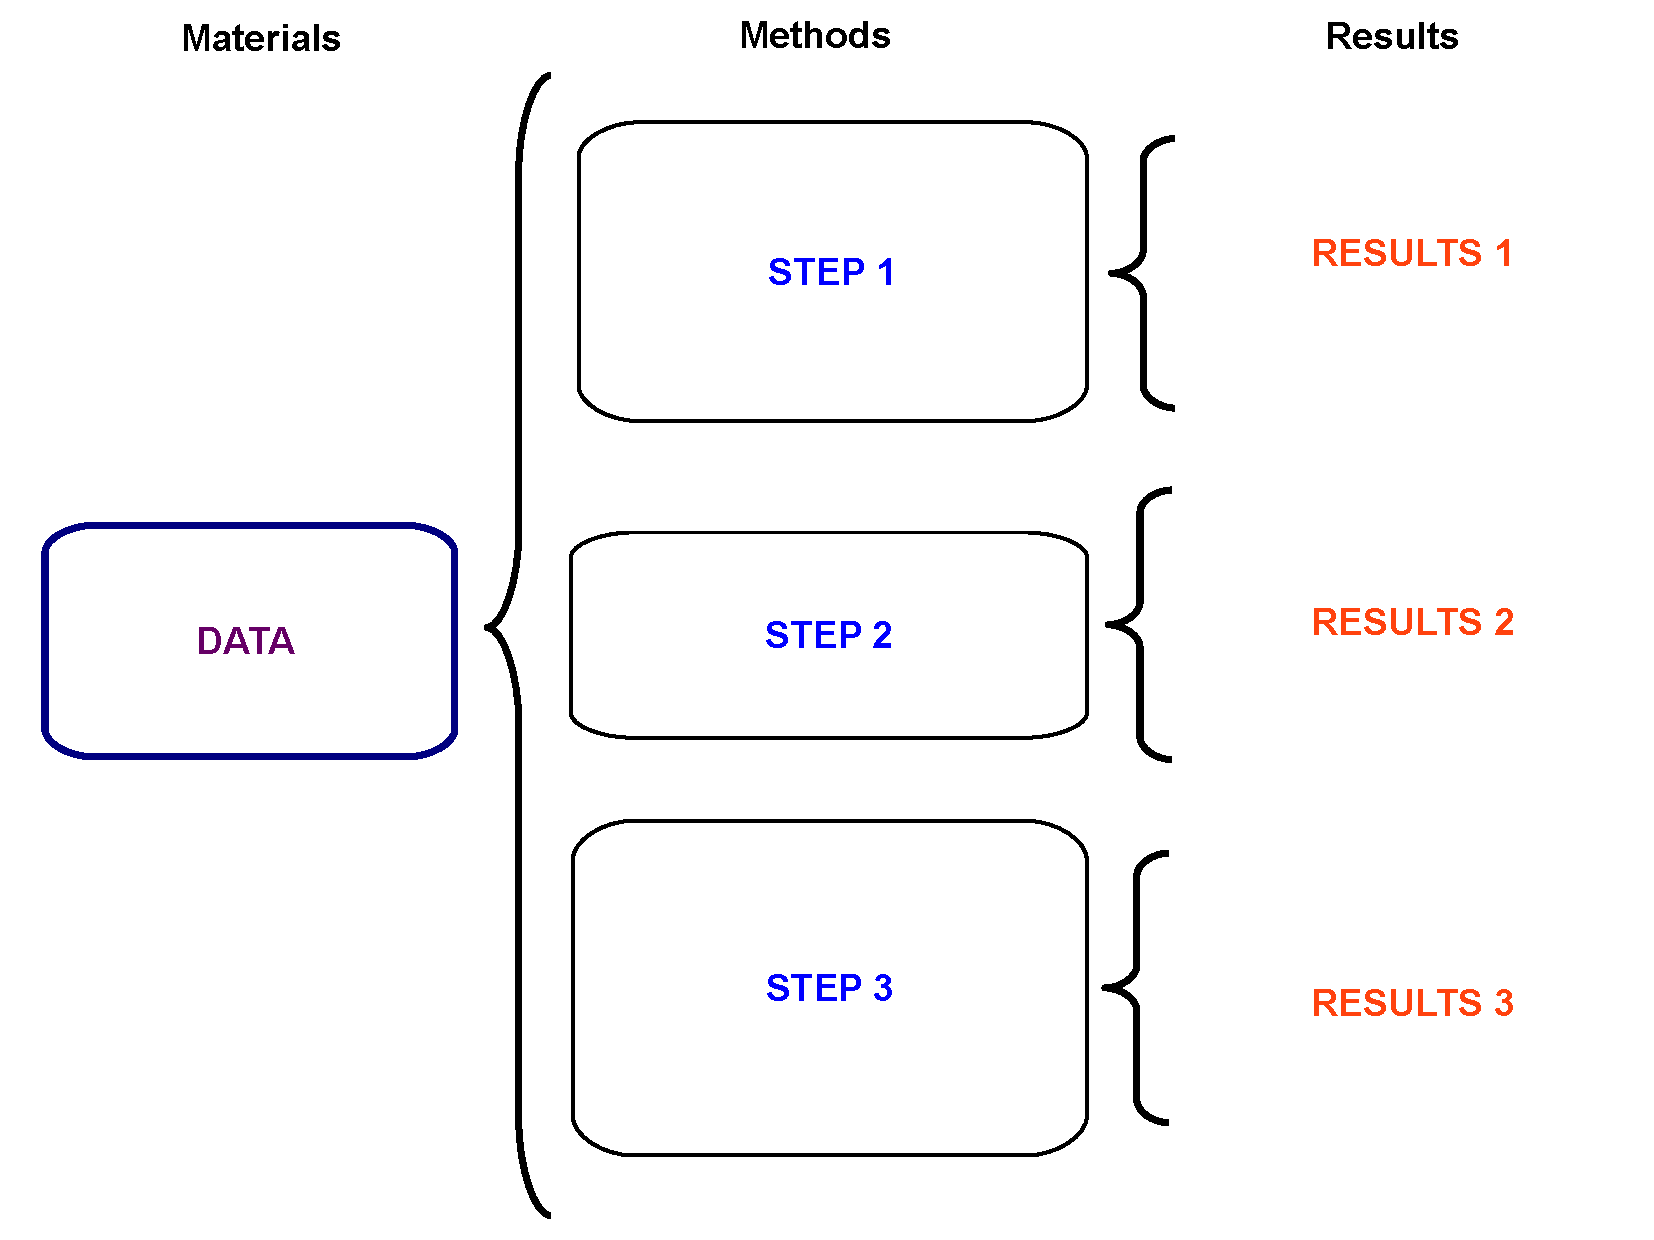
\includegraphics[width=0.9\columnwidth]{materials_and_methods/methods_diagram.pdf}
        \end{center}
    \caption[Flux diagram of general methodology]{
    \textit{\textbf{Flux diagram of general methodology} 
      }
    }
    \label{fig_methods_flux_diagram}    
\end{figure}

